\cotefile{36}
\scanpage{53}
\mspage{-1.6-}

$\phi:V_1\longrightarrow V_2$ commuting with the dual actions, then $\phi\circ E_1=E_2\circ\phi$ where $E_1$ and $E_2$ are the Reynolds operators on $V_{\unsure{1|i}}$ and $V_2$ respectively.

Suppose $V$ is actually a ring $R$, and $\hat\sigma$ is an action on the ring. Then the image of $E$ is\makebox[0pt][r]{\raisebox{-0.55em}[0pt][0pt]{\tikz[x=1em,y=1em]{\draw[line width=.3pt] (0,.04) .. controls (.08,-.02) and (.20,-.02) .. (.28,.05);}}\hspace{.03em}} the subspace of invariant elements of $R$, which is a \uline{subring} $R_0$ of $R$. Although $E$ is not a ring homomorphism, it satisfies the well-known Reynolds identity:
\[
(*)\qquad\text{If }x\in R,\ y\in R_0,\text{ then }E(x.y)=(Ex)\cdot y.
\]
(cf. Cartier\unsure{,} [6], 7-08). To prove this, set $R_1=\ker(E)$. Then $R\cong R_0\oplus R_1$, and $(*)$ is equivalent to the 2 statements $R_0\cdot R_0\subset R_0$ and $R_0\cdot R_1\subset R_1$. To prove the latter, let $g\in R_0$, and let $V\subset R_1$ be a (finite dimensional) irreducible invariant subspace. Then either $g\cdot V=(0)$ or multiplication by $g$ sets up an isomorphism of $V$ with an irreducible invariant subspace $g\cdot V$. Since $g$ is an invariant, the representations of $G$ on $V$ and $g\cdot V$ are isomorphic and non-trivial. Therefore $g\cdot V\subset R_1$.

\begingroup
\setbox0=\hbox{\S2.}
\dimen0=\wd0 \advance\dimen0 by 8pt
\dimen2=\ht0 \advance\dimen2 by \dp0 \advance\dimen2 by 8pt
\leavevmode\rlap{\raisebox{\dimexpr-\dp0-4pt\relax}{%
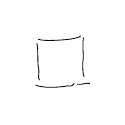
\begin{tikzpicture}[x={\dimexpr\dimen0/105\relax},y={\dimexpr-\dimen2/84\relax},line width=.3pt]
\path[use as bounding box] (0,0) rectangle (105,84);
\draw (16,14) .. controls (23,17) and (55,15) .. (65,14) .. controls (72,13) and (78,12) .. (81,10);
\draw (14,19) .. controls (17,29) and (14,42) .. (17,51) .. controls (18,55) and (15,61) .. (18,64);
\draw (85,12) .. controls (83,24) and (86,33) .. (84,43) .. controls (84,50) and (84,56) .. (86,60);
\draw (12,70) .. controls (23,74) and (48,73) .. (61,71) .. controls (67,72) and (70,70) .. (71,68);
\draw (75,69) .. controls (82,70) and (90,67) .. (95,68);
\end{tikzpicture}}}%
\kern4pt\box0\kern4pt\endgroup With these preliminaries disposed of, we can now take up the first case of the theory - the action of a reductive algebraic group on an affine scheme $X$. To keep straight the techniques in the proof, we do not assume that $X$ is an algebraic scheme over $k$.

\uline{Theorem} \uline{1.1}: Let $X$ be an affine scheme over $k$, let $G$ be a reductive algebraic group, and let $\sigma:G\mathbin{x}X\longrightarrow X$ be an action of $G$ on $X$. Then a universal categorical quotient $(Y,\phi)$ of $X$ by $G$

\margin{52}
